\documentclass[12pt]{beamer}

\usetheme{CambridgeUS}
\usepackage[utf8]{inputenc}
\usepackage{lmodern}
\usepackage{listings}
\usepackage{graphicx}
\usepackage[font=scriptsize,labelfont=bf]{caption}
\usepackage{subcaption}
\usepackage[normalem]{ulem}

\title{Comparativa de sistemes oberts i tancats}

\begin{document}

\frame {
    \maketitle
    \small
    {\centering\itshape Joan Vilà, Sergi Soriano, Miquel Xamani, Arnau Garcia, Guillem Gordillo\par}
}

% Begin Joan Vilà

\frame {
    \frametitle{Instal·lació: temps i problemes}
    \begin{itemize}
        \item {Windows 10}
        \item {Ubuntu}
        \item {Mac OS}
    \end{itemize}
}

\frame {
    \frametitle{Instal·lació de Windows}
    \begin{enumerate}
        \item {Descarregar la ISO (v10 3,71GB)}
        \item {Gravar-la en un CD o USB}
        \item {Reiniciar arrancant des de CD o USB}
        \item {Instal·lar amb siguiente siguiente}
        \item {Aconseguir o tenir una llicència vàlida i demostrar-ho}
    \end{enumerate}
	\begin{center} 
		\begin{figure}
			\centering
			
\includegraphics[width=5cm, height=5cm, keepaspectratio]{windows.png}
		\end{figure}
	\end{center}
}

\frame {
    \frametitle{Instal·lació d'Ubuntu}
    \begin{enumerate}
        \item {Descarregar la ISO (v16.04 1,51GB)}
        \item {Gravar-la en un CD o USB}
        \item {Reiniciar arrancant des de CD o USB}
        \item {Instal·lar amb siguiente siguiente}
    \end{enumerate}
    \begin{center} 
    	\begin{figure}
    		\centering
    		
\includegraphics[width=3cm, height=3cm, keepaspectratio]{ubuntu.png}
    	\end{figure}
    \end{center}
}

\frame {
    \frametitle{Instal·lació de MacOS}
    \begin{enumerate}
        \item {Reiniciar en mode recuperació}
        \item {Seleccionar reinstalar SO}
        \item {Esperar (vSierra 4,86GB)}
    \end{enumerate}
    \begin{center} 
    	\begin{figure}
    		\centering
    		
\includegraphics[width=3cm, height=3cm, keepaspectratio]{apple.png}
    	\end{figure}
    \end{center}
}

\frame {
    \frametitle{Avantatges de cada un}
    \begin{itemize}
        \item {Windows: ???}
        \item {Ubuntu: Gratis, possibilitat d'instal·lar-lo al costat d'altres SO}
        \item {MacOS: Facil, nivell d'usuari baix}
    \end{itemize}
}

\frame {
    \frametitle{Inconvenients de cada un}
    \begin{itemize}
        \item {Windows: Gravar la ISO i el preu/llicència}
        \item {Ubuntu: Gravar la ISO}
        \item {MacOS: Tenir un Mac i temps de descàrrega}
    \end{itemize}
}

\frame {
    \frametitle{Aplicacions disponibles i cost}
    \textbf{Comparació entre Windows Store, Ubuntu Sofware Center i Mac AppStore}
}

\frame {
    \frametitle{Windows Store}
    \begin{itemize}
        \item {669.000 apps per mòbils, ordinadors y tablets}
        \item {Compte! Només aplicacions universals}
    \end{itemize}
    \begin{center} 
    	\begin{figure}
    		\centering
    		
\includegraphics[width=5cm, height=3cm, keepaspectratio]{windowsstore.jpg}
    	\end{figure}
    \end{center}
}

\frame {
    \frametitle{Ubuntu Software Center}
    \begin{itemize}
        \item {Número d'apps desconegut}
        \item {El número depèn de les fonts en les que es confii}
        \item {Possibilitat de posar i traure fonts a gust}
    \end{itemize}
    \begin{center} 
    	\begin{figure}
    		\centering
    		
\includegraphics[width=3cm, height=3cm, keepaspectratio]{ubuntusoftwarecenter.jpg}
    	\end{figure}
    \end{center}
}

\frame {
    \frametitle{Mac App Store}
    \begin{itemize}
        \item {31.191 apps disponibles per a Mac}
        \item {Estricte filtre per penjar una app}
        \item {Traves per a utilitzar apps de tercers}
    \end{itemize}
    \begin{center} 
    	\begin{figure}
    		\centering
    		
\includegraphics[width=3cm, height=3cm, keepaspectratio]{macappstore.png}
    	\end{figure}
    \end{center}
}

\frame {
    \frametitle{Comparació d'alternatives}
    \begin{itemize}
        \item {Windows: Necessitat de buscar la vida per internet}
        \item {Mac: Utilitzar Homebrew com a font de software i buscar la vida per internet}
        \item {Ubuntu: Difícil compatibilitat amb software privatiu de les altres plataformes}
    \end{itemize}
}

\frame {
    \frametitle{Comparativa de preus}
    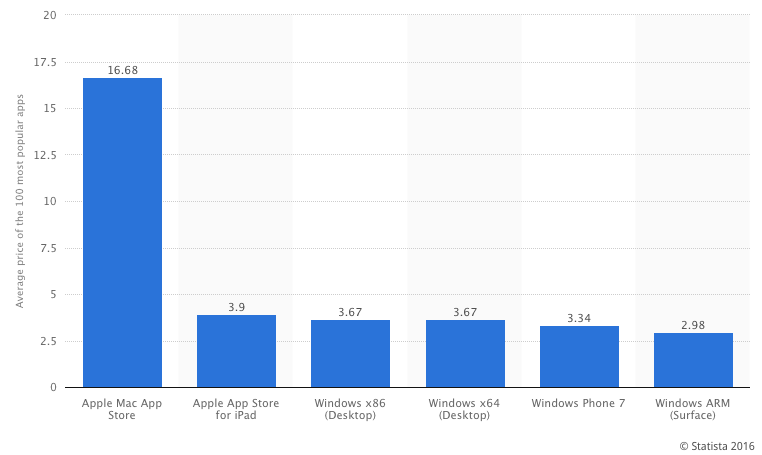
\includegraphics[width=\textwidth]{PriceComparison.png}
}

\frame {
    \frametitle{Reflexió de problemes vistos fins el moment}
    \begin{itemize}
        \item {Windows: Software propens a virus i amb problemes de privacitat}
        \item {Mac: Hacks com Homebrew per accedir a fonts de software i problemes de privacitat}
        \item {Ubuntu: No és posible utilitzar sofware popular de Microsoft, Adobe...}
    \end{itemize}
}

\frame {
	\frametitle{Software privatiu i sofware lliure}
	\begin{itemize}
		\item {Alternatives lliures més populars que privatives (Gimp, Firefox, VLC, Thunderbird...)}
		\item {Cada dia més aplicacions funcionen en linux (Spotify, Dropbox, Atom, Chrome...)}
		\item {Esque jo vull Photoshop... wine}
	\end{itemize}
}

\frame {
	\frametitle{Requisits per fer arribar Linux al públic}
	\begin{itemize}
		\item{Que es desenvolupi per a Linux com es fa per Windows o Mac}
		\item{El software d'empresa tradicional estigui disponible}
		\item{Que un usuari normal no hagi de fer servir la terminal}
	\end{itemize}
}

% End Joan Vilà
% Begin Sergi Soriano

\frame {
    \frametitle{Comparativa de velocitats entre els sistemes operatius}
    \begin{itemize}
        \item{Boot}
        \item{Aplicacions}
        \item{Còpies de fitxers}
    \end{itemize}
}

\frame {
    \frametitle{Comparativa de velocitat entre els sistemes operatius}
    \begin{itemize}
        \item{Windows 10}
        \item{Ubuntu 16.04}
        \item{macOS Sierra}
    \end{itemize}
}

\frame {
    \frametitle{Comparativa de velocitat entre els sistemes operatius}
    \framesubtitle{Entorn}
    \begin{itemize}
        \item{Processador AMD FX-6300}
        \item{MSI 970A-G46}
        \item{4 GB de RAM}
        \item{60 GB de disc dur}
    \end{itemize}
}

\frame {
    \frametitle{Comparativa de velocitats entre els sistemes operatius}
    \begin{itemize}
        \item{Windows 10}
        \item{Ubuntu 16.04}
        \item
        \sout{macOS Sierra}
    \end{itemize}    
}

\frame {
    \frametitle{Comparativa de velocitats entre els sistemes operatius}
    \begin{figure}
        \centering
        
\includegraphics[height=2cm, keepaspectratio]{media_aritmetica.png}
    \end{figure}  
}

\frame {
    \frametitle{Comparativa de velocitats entre els sistemes operatius}
    \begin{itemize}
        \item{\textbf{Boot}}
        \item{Aplicacions}
        \item{Còpies de fitxers}
    \end{itemize}
}

\frame {
    \frametitle{Comparativa de velocitat entre els sistemes operatius}
    \framesubtitle{Velocitat d'arrancada}
    \begin{figure}
        \centering
        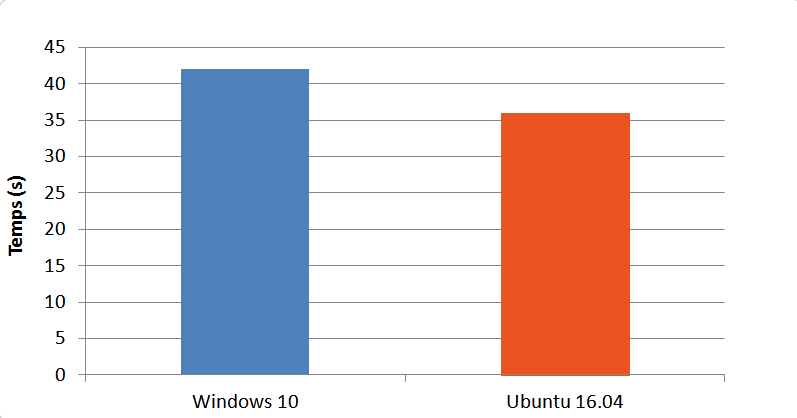
\includegraphics[height=5cm, keepaspectratio]{comparativaArrancada.png}
        \caption{Temps de boot del sistema}
    \end{figure}
}

\frame {
    \frametitle{Comparativa de velocitats entre els sistemes operatius}
    \begin{itemize}
        \item{Boot}
        \item{\textbf{Aplicacions}}
        \item{Còpies de fitxers}
    \end{itemize}
}

\frame {
    \frametitle{Comparativa de velocitat entre aplicacions}
    \framesubtitle{Execució d'aplicacions}
    \begin{columns}[t]
        \column{.5\textwidth}
            \centering
            
\includegraphics[width=5cm,height=3cm, keepaspectratio]{firefox_logo.png}\\
            
\includegraphics[width=5cm,height=3cm, keepaspectratio]{chrome_logo.png}
        \column{.5\textwidth}
            \centering
            
\includegraphics[width=5cm,height=3cm, keepaspectratio]{skype_logo.png}\\
            
\includegraphics[width=5cm,height=3cm, keepaspectratio]{steam_logo.png}
        \end{columns}
}

%Firefox
\frame {
    \frametitle{Comparativa en aplicacions - Firefox}
    \begin{figure}
        \centering
        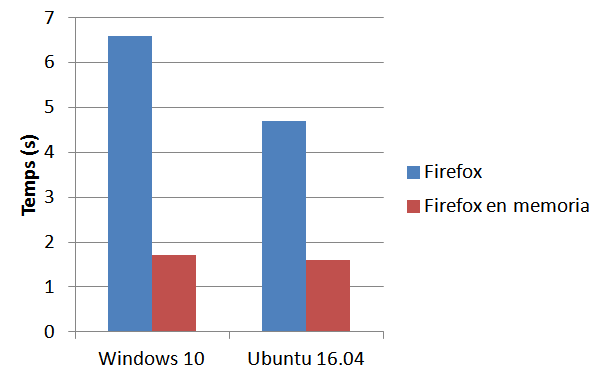
\includegraphics[height=5cm, keepaspectratio]{comparativa_firefox.png}
        \caption{Temps d'execució de Firefox}
    \end{figure}
}

%Chrome
\frame {
    \frametitle{Comparativa en aplicacions - Chrome}
    \begin{figure}
        \centering
        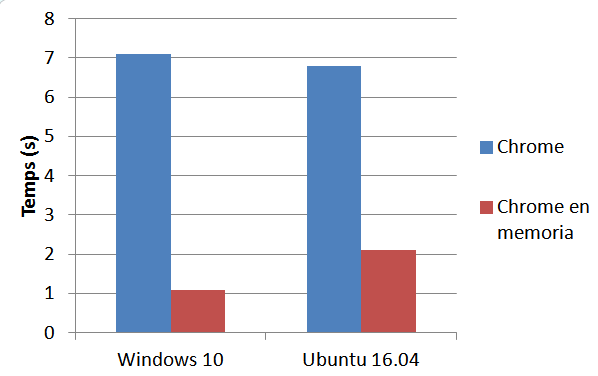
\includegraphics[height=5cm, keepaspectratio]{comparativa_chrome.png}
        \caption{Temps d'execució de Chrome}
    \end{figure}
}

%Skype
\frame {
    \frametitle{Comparativa en aplicacions - Skype}
    \begin{figure}
        \centering
        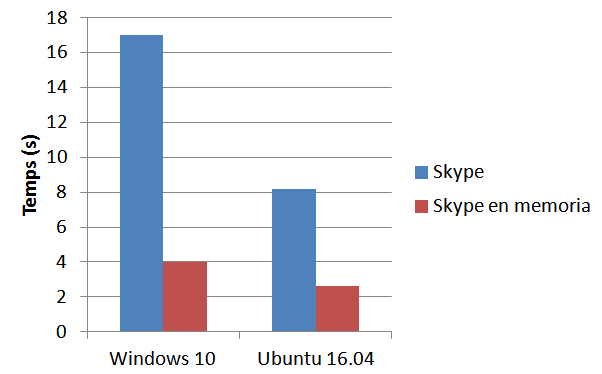
\includegraphics[height=5cm, keepaspectratio]{comparativa_skype.png}
        \caption{Temps d'execució de Skype}
    \end{figure}
}

%Steam
\frame {
    \frametitle{Comparativa en aplicacions - Steam}
    \begin{figure}
        \centering
        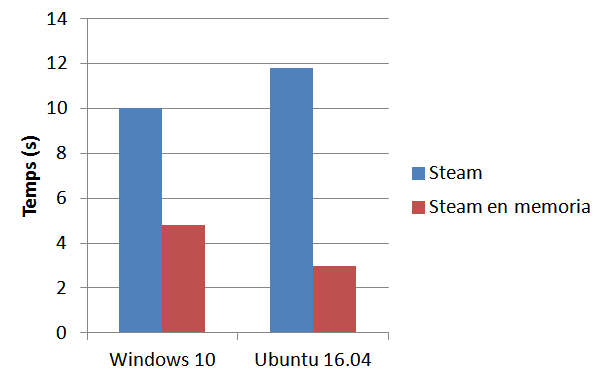
\includegraphics[height=5cm, keepaspectratio]{comparativa_steam.png}
        \caption{Temps d'execució de Steam}
    \end{figure}
}

\frame {
    \frametitle{Comparativa de velocitats entre els sistemes operatius}
    \begin{itemize}
        \item{Boot}
        \item{Aplicacions}
        \item{\textbf{Còpies de fitxers}}
    \end{itemize}
}

%copies de fitxers
\frame {
    \frametitle{Velocitat en còpies de fitxers}
    \begin{itemize}
        \item{Fitxer únic (2,4 GB)}
        \item{Conjunt de fitxers (2.44 GB)}
    \end{itemize}
}

\frame {
    \frametitle{Fitxer únic}
    \underline{Windows 10}
    \begin{itemize}
        \item{Velocitat aproximada: 37 MB/s}
        \item{Temps: 1 min. 10 s}
    \end{itemize}
    
    \underline{Ubuntu 16.04}
    \begin{itemize}
        \item{Velocitat aproximada: 70 MB/s}
        \item{Temps: 40 s}
    \end{itemize}
}

\frame {
    \frametitle{Conjunt de fitxers}
    \underline{Windows 10}
    \begin{itemize}
        \item{Velocitat aproximada: 50 - 20 MB/s}
        \item{Temps: 1 min}
    \end{itemize}
    
    \underline{Ubuntu 16.04}
    \begin{itemize}
        \item{Velocitat aproximada: 60 - 25 MB/s}
        \item{Temps: 50 s}
    \end{itemize}
}

\frame {
    \frametitle{Conclusions}
    \begin{itemize}
        \item{Ubuntu guanya la comparativa de boot del sistema.}
        \item{Tant Windows com Ubuntu són molt ràpids quan tenen el programa en memòria}
    \end{itemize}
}


% End Sergi Soriano
% Begin Miquel Xamani
\frame {
	\frametitle{Comparativa entre servidors NFS Windows i Linux}
	\framesubtitle{Entorn}
	\underline{Client}
	\vspace{2mm}
	\begin{itemize}
		\item{Benchmarks executats des d’un client Linux CentOS 7.1}
	\end{itemize}
	\vspace{5mm}
	\underline{Servidor}
	\vspace{2mm}
	\begin{itemize}
		\item{Servidor NFS Linux CentOS 7.1}
		\item{Servidor NFS Windows 2012 Data Center Edition}
		\item{\textbf{Igualtat de condicions} $\rightarrow$ Els 2 servidors tenen 2GB de RAM, 2 cores,  exactament el mateix hardware,  mateixa versió de NFS (4.1), 40 GB de disc assignats exclusivament pel benchmark i tenen un disc secundari per les accions del SO.}
	\end{itemize}
}

\frame {
	\frametitle{Comparativa entre servidors NFS Windows i Linux}
	\framesubtitle{Test}
	S'ha utilitzat \textbf{IOZone Benchmark} per mesurar les operacions:
	\vspace{3mm}
	\begin{itemize}
		\item{Sequential Write}
		\item{Sequential Read}
		\item{Random Write}
		\item{Random Read}
	\end{itemize}
}

\frame {
	\frametitle{Comparativa entre servidors NFS Windows i Linux}
	\framesubtitle{Resultats}
	\underline{Mètriques}
	\vspace{3mm}
	\begin{itemize}
		\item{\textbf{File size}: tamany del fitxer llegit/escrit}
		\item{\textbf{Record size}: tamany de la partició que constitueix un fitxer}
		\item{\textbf{MBps}: velocitat en què un fitxer és llegit/escrit de disc}
	\end{itemize}
}

\frame {
    \frametitle{Comparativa entre servidors NFS Windows i Linux}
    \framesubtitle{Resultats Sequential Write}
      \begin{figure}
        \begin{subfigure}[b]{0.3\textwidth}
          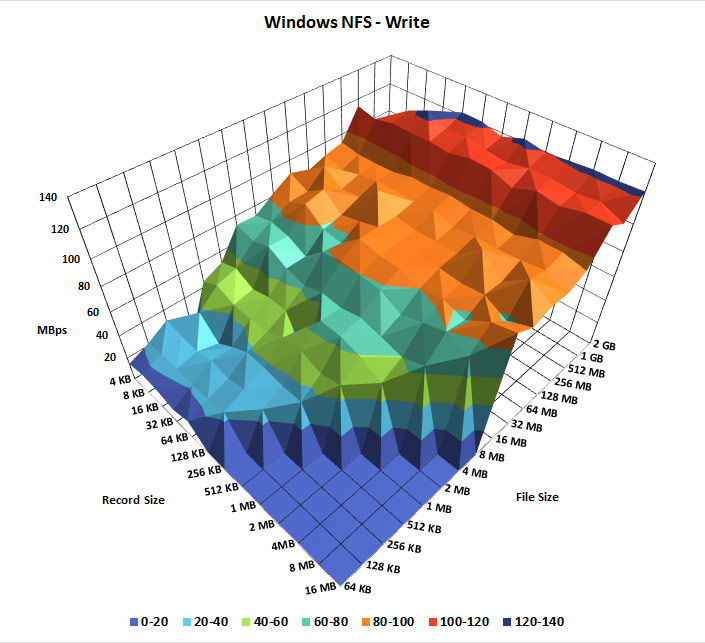
\includegraphics[width=6cm, height=8cm, keepaspectratio]{windows-nfs-write.jpg}
        \end{subfigure}
        \hspace*{\fill}
        \begin{subfigure}[b]{0.3\textwidth}
          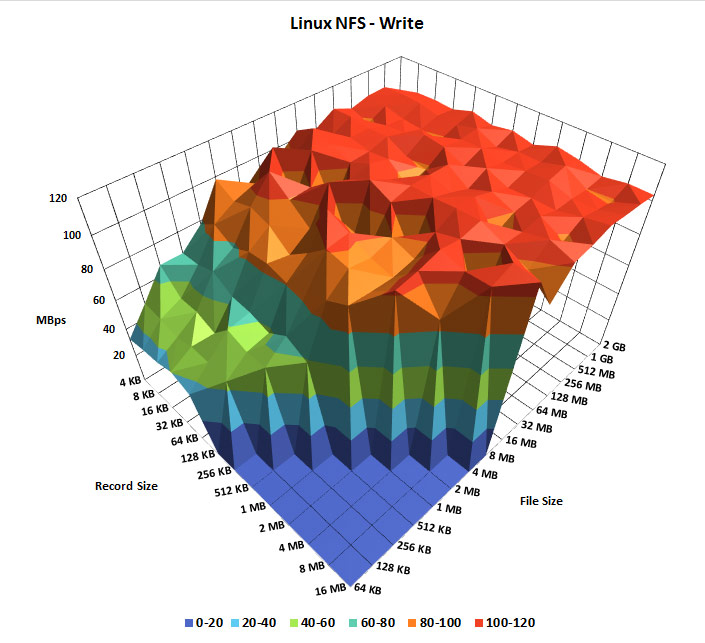
\includegraphics[width=6cm, height=8cm, keepaspectratio]{linux-nfs-write.jpg}
        \end{subfigure}
        \hspace*{\fill}
      \end{figure}
}

\frame {
    \frametitle{Comparativa entre servidors NFS Windows i Linux}
    \framesubtitle{Resultats Sequential Read}
      \begin{figure}
        \begin{subfigure}[b]{0.3\textwidth}
          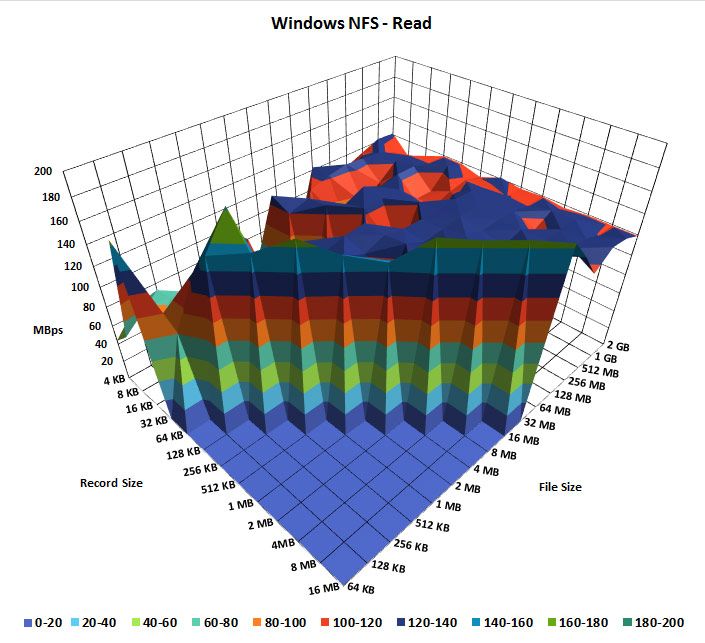
\includegraphics[width=6cm, height=8cm, keepaspectratio]{windows-nfs-read.jpg}
        \end{subfigure}
        \hspace*{\fill}
        \begin{subfigure}[b]{0.3\textwidth}
          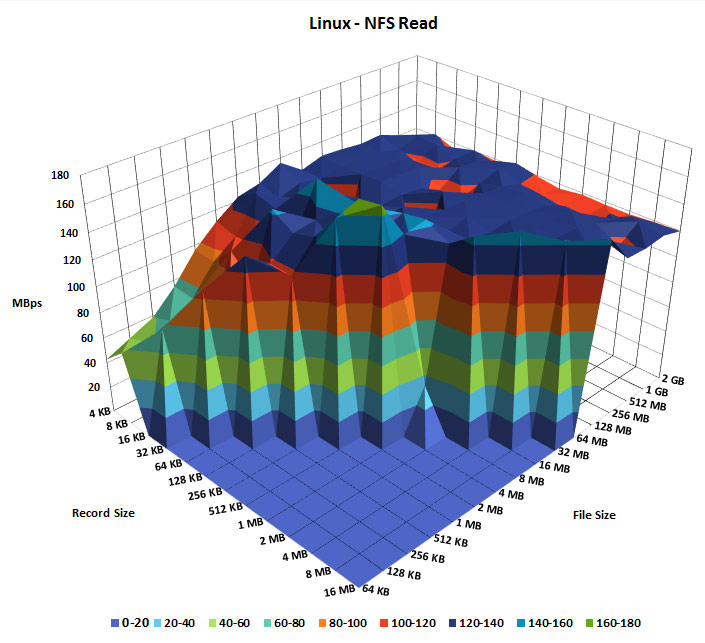
\includegraphics[width=6cm, height=8cm, keepaspectratio]{linus-nfs-read.jpg}
        \end{subfigure}
        \hspace*{\fill}
      \end{figure}
}

\frame {
    \frametitle{Comparativa entre servidors NFS Windows i Linux}
    \framesubtitle{Resultats Random Write}
      \begin{figure}
        \begin{subfigure}[b]{0.3\textwidth}
          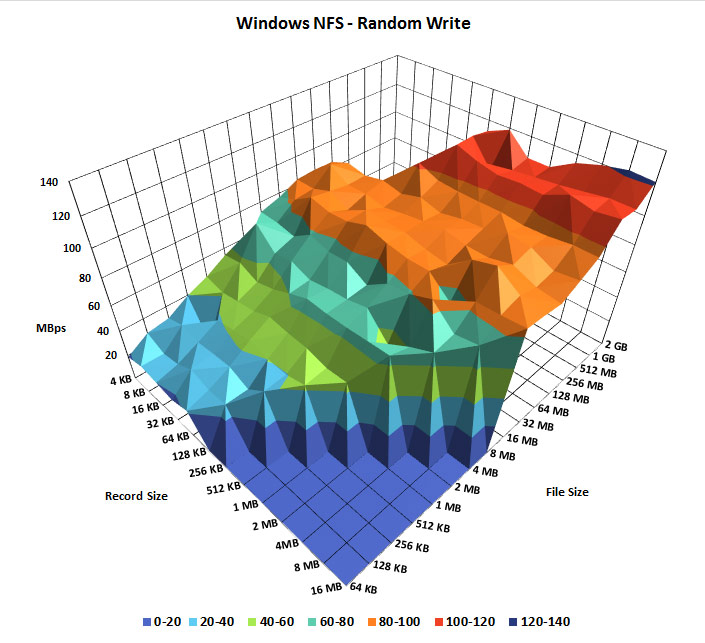
\includegraphics[width=6cm, height=8cm, keepaspectratio]{windows-nfs-random-write.jpg}
        \end{subfigure}
        \hspace*{\fill}
        \begin{subfigure}[b]{0.3\textwidth}
          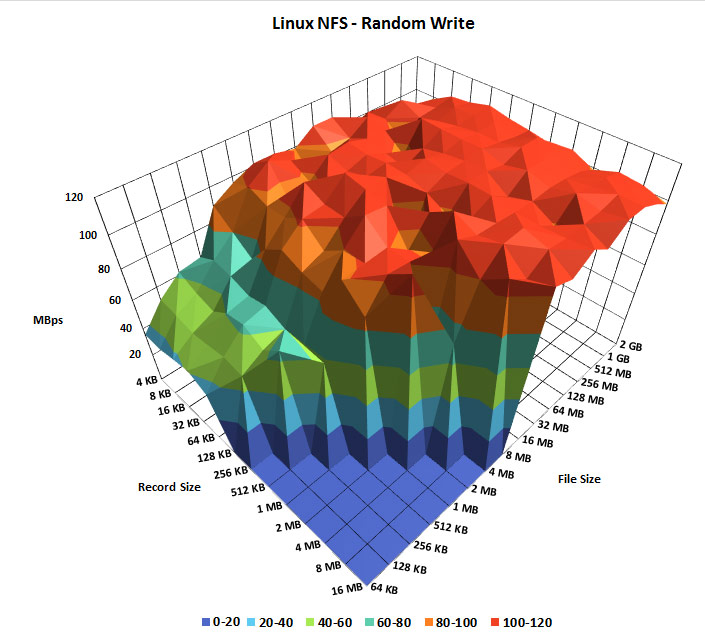
\includegraphics[width=6cm, height=8cm, keepaspectratio]{linux-nfs-random-write.jpg}
        \end{subfigure}
        \hspace*{\fill}
      \end{figure}
}

\frame {
    \frametitle{Comparativa entre servidors NFS Windows i Linux}
    \framesubtitle{Resultats Random Write}
      \begin{figure}
        \begin{subfigure}[b]{0.3\textwidth}
          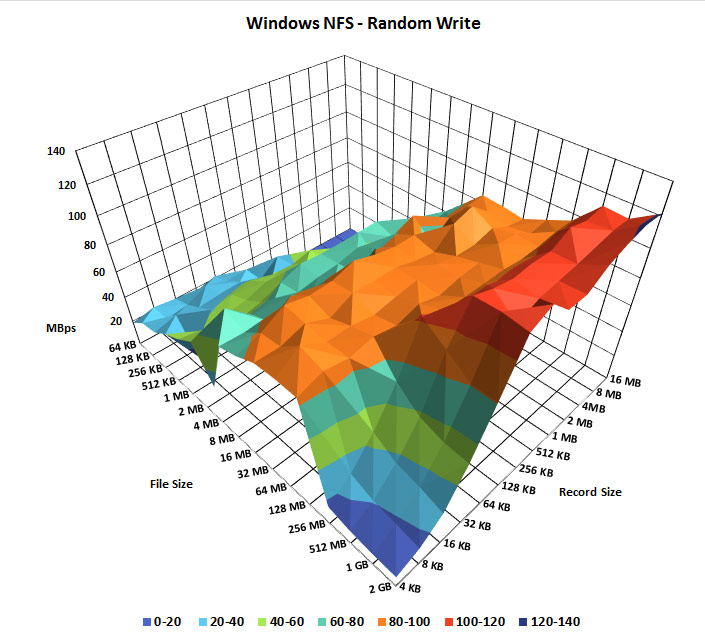
\includegraphics[width=6cm, height=8cm, keepaspectratio]{windows-nfs-random-write2.jpg}
        \end{subfigure}
        \hspace*{\fill}
        \begin{subfigure}[b]{0.3\textwidth}
          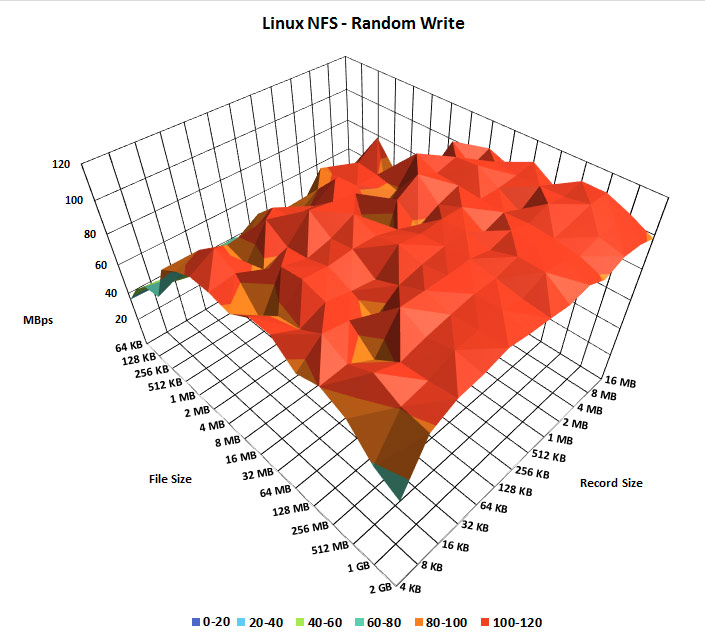
\includegraphics[width=6cm, height=8cm, keepaspectratio]{linux-nfs-random-write2.jpg}
        \end{subfigure}
        \hspace*{\fill}
      \end{figure}
}

\frame {
    \frametitle{Comparativa entre servidors NFS Windows i Linux}
    \framesubtitle{Resultats Random Read}
      \begin{figure}
        \begin{subfigure}[b]{0.3\textwidth}
          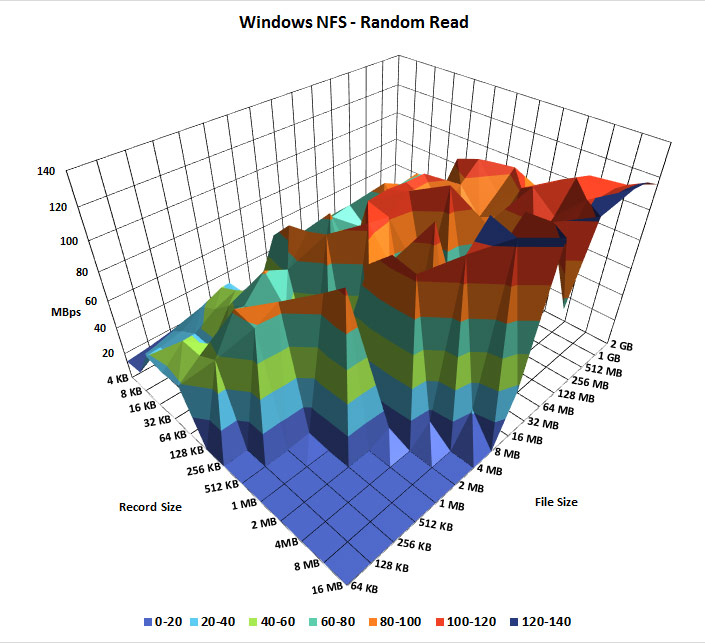
\includegraphics[width=6cm, height=8cm, keepaspectratio]{windows-nfs-random-read.jpg}
        \end{subfigure}
        \hspace*{\fill}
        \begin{subfigure}[b]{0.3\textwidth}
          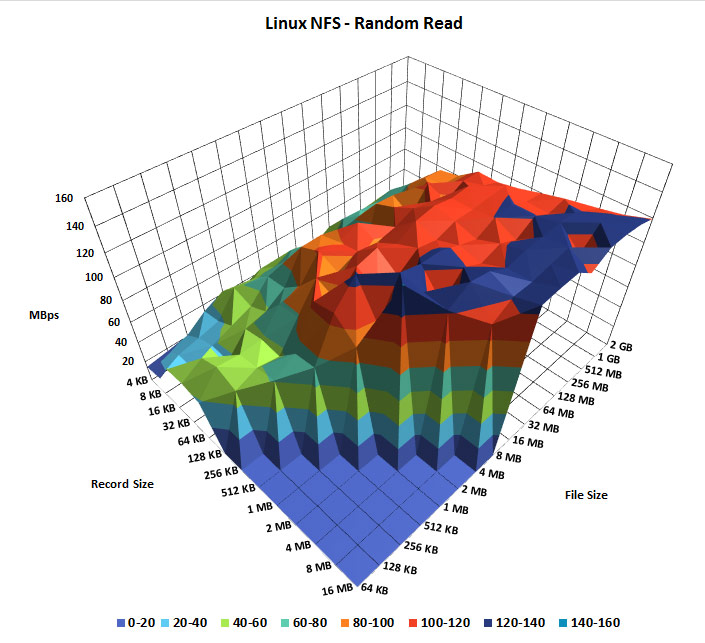
\includegraphics[width=6cm, height=8cm, keepaspectratio]{linux-nfs-random-read.jpg}
        \end{subfigure}
        \hspace*{\fill}
      \end{figure}
}

\frame {
	\frametitle{Comparativa entre servidors NFS Windows i Linux}
	\framesubtitle{Conclusió}
	\underline{Conclusió}\\
	\vspace{3mm}
	\textbf{El servidor Linux ofereix millor rendiment i és més constant que Windows en la majoria de tests.}
}

\frame {
    \frametitle{Ús de recursos del sistema}
    \framesubtitle{Monitoritzar l’ús dels recursos del sistema a Windows}
    \begin{itemize}
    \item{Administrador de tasques}
    \end{itemize}
    \begin{center} 
      \begin{figure}
        \centering
        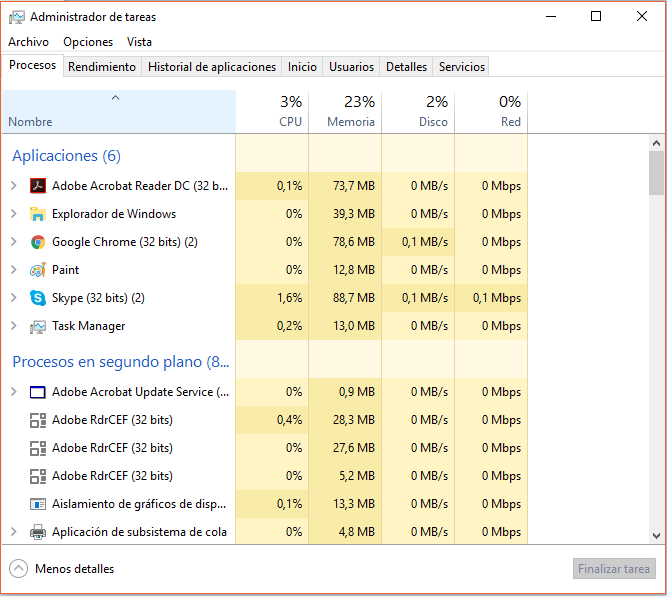
\includegraphics[width=7cm, height=5cm, keepaspectratio]{administrador_tasques.png}
        \caption{Administrador de tasques a Windows 10}
      \end{figure}
    \end{center}
}

\frame {
    \frametitle{Ús de recursos del sistema}
    \framesubtitle{Monitoritzar l’ús dels recursos del sistema a Windows}
    \begin{itemize}
    \item{Administrador de tasques}
    \item{Eines de tercers com System Explorer o CPU-Z}
    \end{itemize}
    \begin{center} 
      \begin{figure}
        \centering
        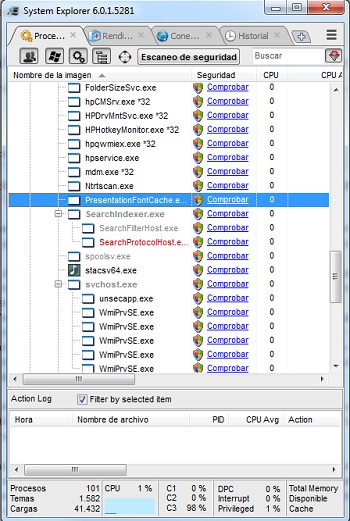
\includegraphics[width=7cm, height=5cm, keepaspectratio]{systemexplorer.jpg}
        \caption{System explorer}
      \end{figure}
    \end{center}
}

\frame {
    \frametitle{Ús de recursos del sistema}
    \framesubtitle{Monitoritzar l’ús dels recursos del sistema a Ubuntu}
    \begin{itemize}
    \item{Línia de comandes (top, free, vmstat, iostat, ps, du, df ...)}
    \end{itemize}
    \begin{center} 
      \begin{figure}
        \begin{subfigure}[b]{0.3\textwidth}
          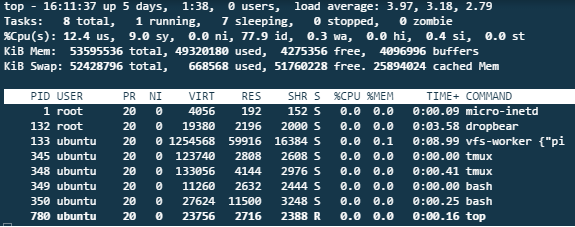
\includegraphics[width=4cm, height=3cm, keepaspectratio]{top_command.png}
          \caption{Sortida comanda top}
        \end{subfigure}
        \qquad
        \begin{subfigure}[b]{0.3\textwidth}
          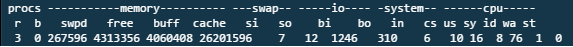
\includegraphics[width=5.5cm, height=4cm, keepaspectratio]{vmstat_command.png}
          \caption{Sortida comanda vmstat}
        \end{subfigure}
      \end{figure}
    \end{center}
}

\frame {
    \frametitle{Ús de recursos del sistema}
    \framesubtitle{Monitoritzar l’ús dels recursos del sistema a Ubuntu}
    \begin{itemize}
    \item{Línia de comandes (top, free, vmstat, iostat, ps, du, df ...)}
    \item{Monitor del sistema}
    \end{itemize}
    \begin{center} 
      \begin{figure}
        \centering
        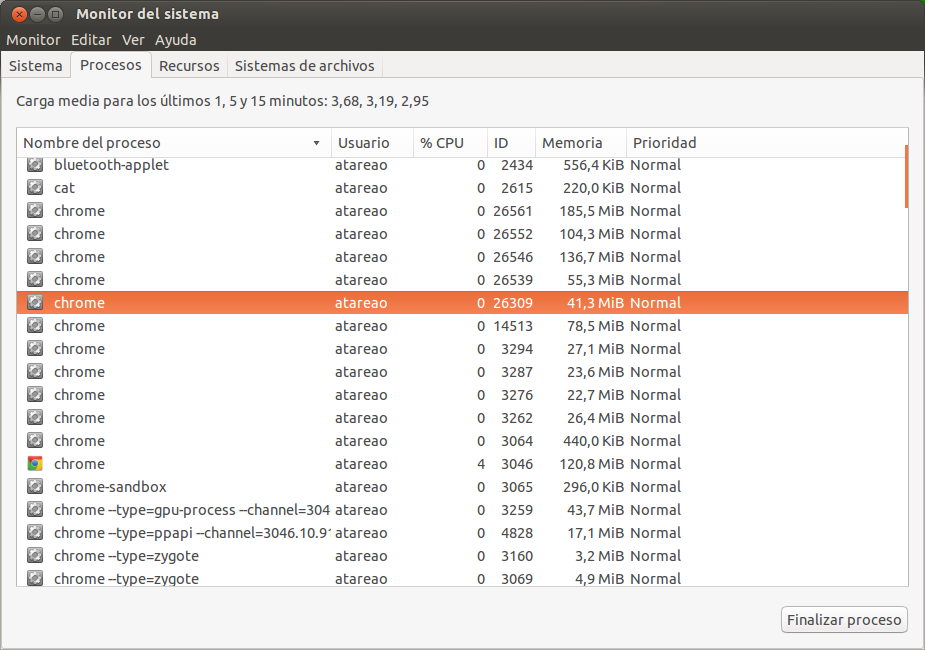
\includegraphics[width=7cm, height=4cm, keepaspectratio]{monitor_del_sistema.png}
        \caption{Monitor del sistema}
      \end{figure}
    \end{center}
}

\frame {
    \frametitle{Ús de recursos del sistema}
    \framesubtitle{Monitoritzar l’ús dels recursos del sistema a Ubuntu}
    \begin{itemize}
    \item{Línia de comandes (top, free, vmstat, iostat, ps, du, df ...)}
    \item{Monitor del sistema}
    \item{Eines de tercers com I-Nex o Conky}
    \end{itemize}
    \begin{center} 
      \begin{figure}
        \centering
        \begin{subfigure}[b]{0.3\textwidth}
          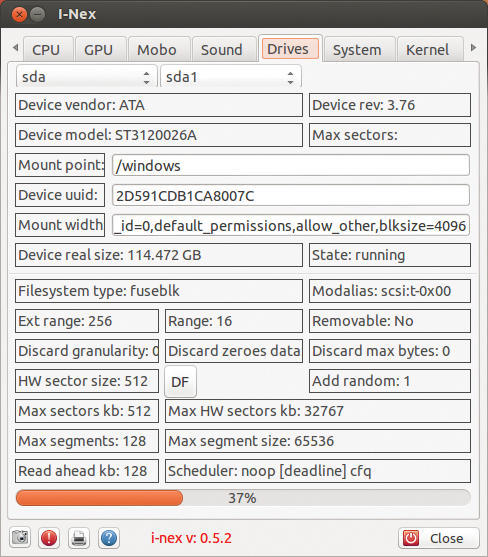
\includegraphics[width=\textwidth]{i-nex_drive_reference.jpg}
          \caption{I-Nex}
        \end{subfigure}
        \qquad
        \begin{subfigure}[b]{0.3\textwidth}
          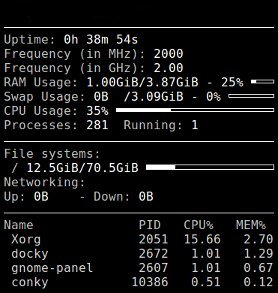
\includegraphics[width=\textwidth]{conky-por-defecto.jpg}
          \caption{Conky per defecte}
        \end{subfigure}
      \end{figure}
    \end{center}
}

\frame {
    \frametitle{Ús de recursos del sistema}
    \framesubtitle{Monitoritzar l’ús dels recursos del sistema a MacOS}
    \begin{itemize}
    \item{Monitor de actividad}
    \end{itemize}
    \begin{center} 
      \begin{figure}
        \centering
        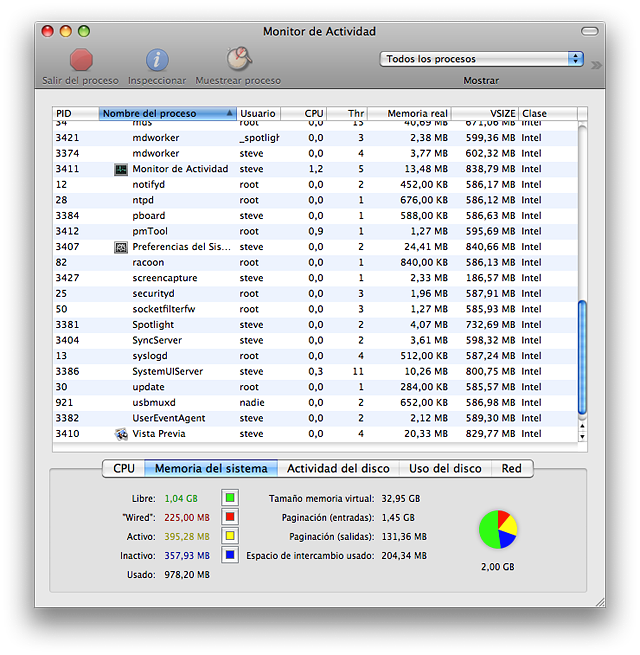
\includegraphics[width=7cm, height=4cm, keepaspectratio]{activity_monitor.png}
        \caption{Monitor de actividad}
      \end{figure}
    \end{center}
}

\frame {
    \frametitle{Ús de recursos del sistema}
    \framesubtitle{Monitoritzar l’ús dels recursos del sistema a MacOS}
    \begin{itemize}
    \item{Monitor de actividad}
    \item{Eines de tercers com iStat Menus i StatsBar}
    \end{itemize}
    \begin{center} 
      \begin{figure}
        \centering
        \begin{subfigure}[b]{0.3\textwidth}
          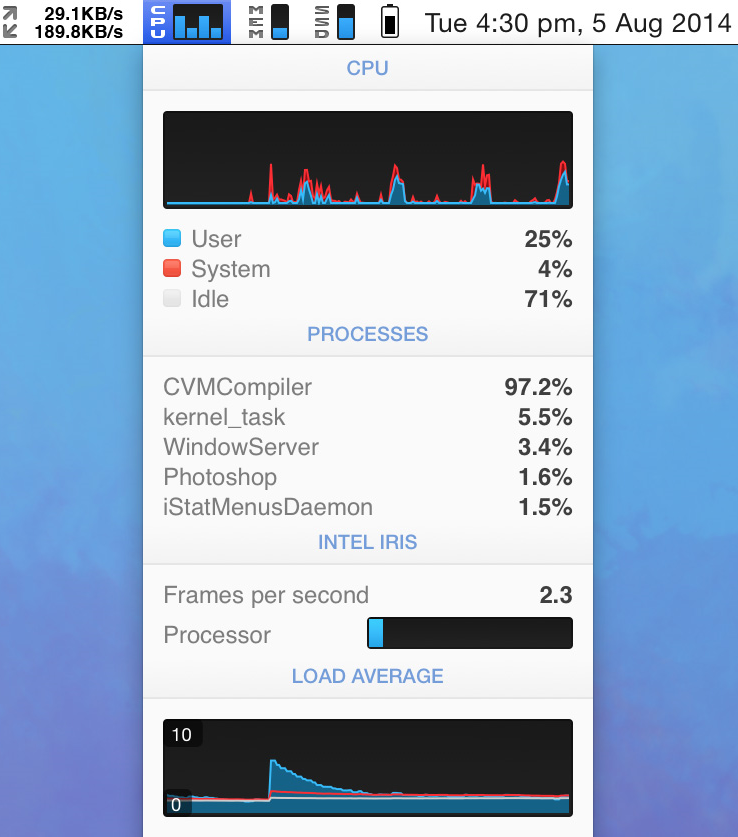
\includegraphics[width=5cm, height=4cm, keepaspectratio]{istat_menus.png}
          \caption{iStat Menus}
        \end{subfigure}
        \qquad
        \begin{subfigure}[b]{0.3\textwidth}
          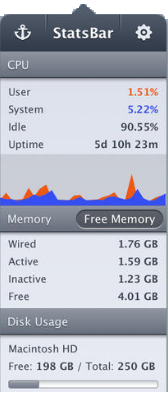
\includegraphics[width=3cm, height=4cm, keepaspectratio]{statsbar.png}
          \caption{StatsBar}
        \end{subfigure}
      \end{figure}
    \end{center}
}

\frame {
    \frametitle{Ús de recursos del sistema}
    \framesubtitle{Requisits mínims}
    \begin{center} 
      \begin{figure}
        \centering
        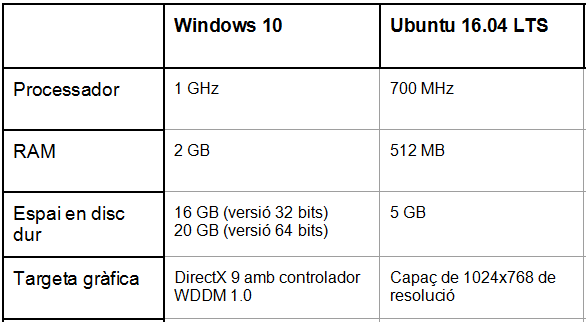
\includegraphics[width=9cm, height=6cm, keepaspectratio]{requisits_minims1.png}
        \caption{Requisits mínims Windows 10 i Ubuntu 16.04 LTS}
      \end{figure}
    \end{center}
}

\frame {
    \frametitle{Ús de recursos del sistema}
    \framesubtitle{Requisits mínims}
    \begin{center} 
      \begin{figure}
        \centering
        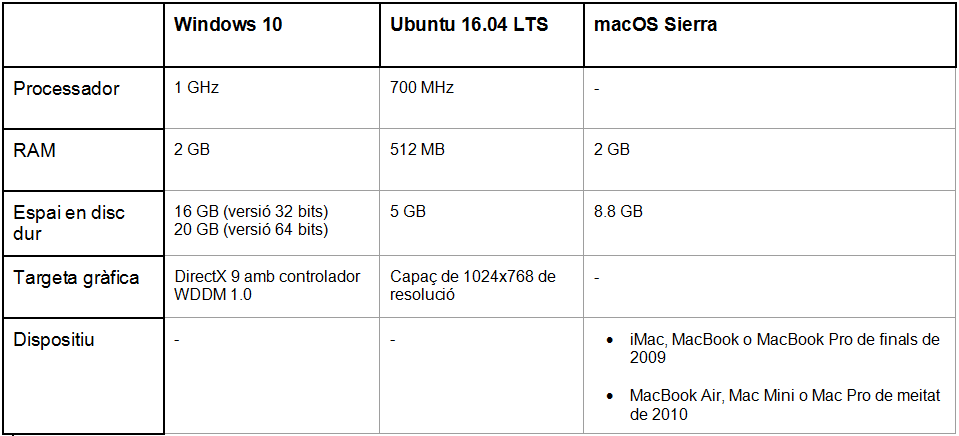
\includegraphics[width=10cm, height=7cm, keepaspectratio]{requisits_minims2.png}
        \caption{Requisits mínims Windows 10, Ubuntu 16.04 LTS i MacOS Sierra}
      \end{figure}
    \end{center}
}

\frame {
    \frametitle{Ús de recursos del sistema}
    \framesubtitle{Ús d'espai de disc}
    \begin{center} 
      \begin{figure}
        \centering
        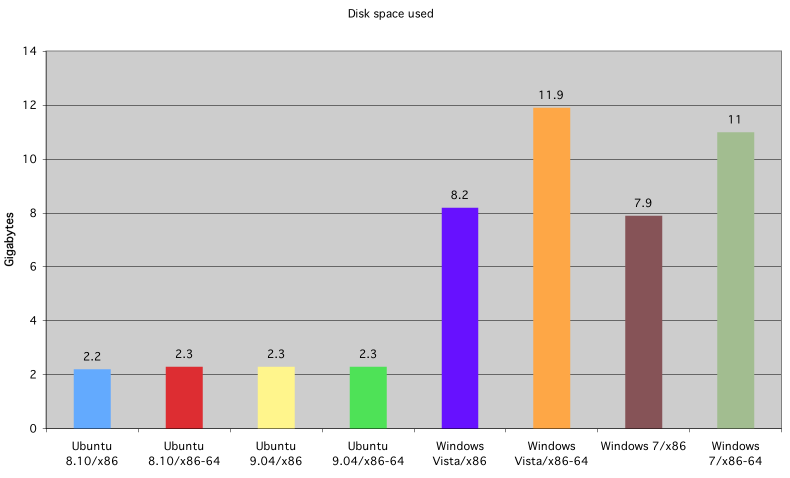
\includegraphics[width=9cm, height=6cm, keepaspectratio]{disk_space_usage.png}
        \caption{Ús d'espai de disc de versions d'Ubuntu i Windows antigues}
      \end{figure}
    \end{center}
}


% End Miquel Xamani
% Begin Arnau Garcia

\frame {
    \frametitle{Comparativa de tiempos/recursos para una aplicación en el mismo PC bajo distintos SO}
    \framesubtitle{Introducció}
    \begin{itemize}
    \item {Interacció entre els components del sistema operatiu i el temps d'execució segueix sent en part un misteri}
    \end{itemize}
    \begin{enumerate}
    \item{Fallades de la memòria de traducció (TLB)}
    \item{Interrupcions}
    \item{Events asíncrons}
    \end{enumerate}
    \begin{itemize}
    \item{Poden \textbf{afectar el rendiment} dels SO}
    \end{itemize}
}
\frame {
    \frametitle{Comparativa de tiempos/recursos para una aplicación en el mismo PC bajo distintos SO}
    \framesubtitle{Introducció}
    \begin{itemize}
    \item {\textbf{Soroll}: interferència del sistema operatiu}
    \item{Important intentar definir/interpretar el que es considera soroll:}
    \end{itemize}
    \begin{center}
    \large{\emph{"Col·lecció d'activitats de fons que involuntàriament interrumpeixen el progrés de l'aplicació principal.”}}
    \end{center}
}
\frame {
    \frametitle{Comparativa de tiempos/recursos para una aplicación en el mismo PC bajo distintos SO}
    \framesubtitle{Simulació 1 - Factorial}
    \begin{itemize}
    \item {Sistemes operatius:}
	\begin{itemize}
	\item\textbf{openSUSE 13.2 (Harlequin) (64 bits)}
    	\item\textbf{Windows 7 ENTERPRISE (64 bits)}
    	\end{itemize}
    \item {Medició:}
	\begin{itemize}
	\item\textbf{Factorial de 10}
    	\end{itemize}
    \item {Processador:}
	\begin{itemize}
	\item\textbf{Intel(R) Core(TM) i5-3470 CPU @ 3.20GHz - 64 bits}
    	\end{itemize}
    \item {Memòria RAM:}
	\begin{itemize}
	\item\textbf{8 GB}
    	\end{itemize}
    \item {Nom de l'equip:}
	\begin{itemize}
	\item\textbf{c6s301pc42}
    	\end{itemize}
    \item {Domini:}
	\begin{itemize}
	\item\textbf{FIBSMB}
    	\end{itemize}
    \end{itemize}
}

\begin{frame}[fragile]
\frametitle{Comparativa de tiempos/recursos para una aplicación en el mismo PC bajo distintos SO}
\framesubtitle{Simulació 1 - Factorial}
\textbf{openSUSE}	     
  \begin{lstlisting}
 #!/bin/bash
START="$(($(date +%s%N)/1000000))"
cd /home/Desktop/
./factorial.out
END="$(($(date +%s%N)/1000000))" 
TOTAL=$(($END-$START))
echo "END: "$END "START: "$START "TOTAL: "$TOTAL
    \end{lstlisting}
\end{frame}

\frame {
    \frametitle{Comparativa de tiempos/recursos para una aplicación en el mismo PC bajo distintos SO}
    \framesubtitle{Simulació 1 - Factorial}

  \begin{tabular}{cl}  
         \begin{tabular}{c}
           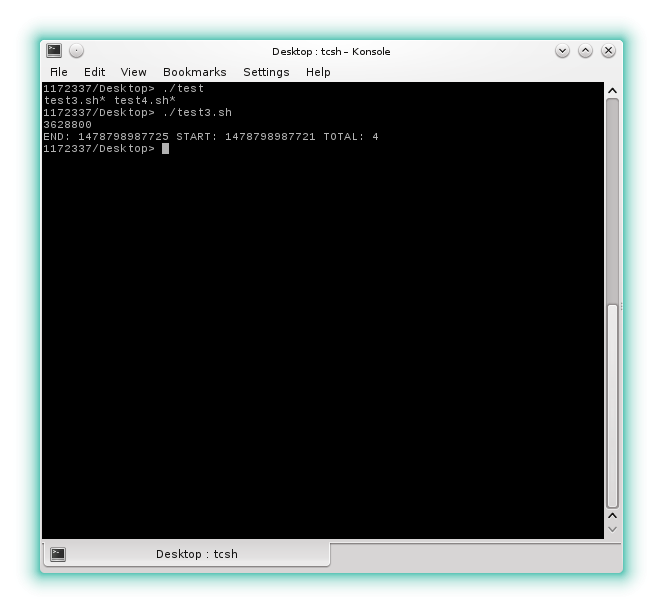
\includegraphics[height=8cm, width=7cm]{factorial_open_suse.png}
           \end{tabular}
           & \begin{tabular}{l}
             \parbox{0.5\linewidth}{
	     \begin{itemize}
             \item\textbf{openSUSE}
	     \item\textbf{4 Mil·lisegons}
	     \end{itemize}}
         \end{tabular}  \\
\end{tabular}
}
\begin{frame}[fragile]
\frametitle{Comparativa de tiempos/recursos para una aplicación en el mismo PC bajo distintos SO}
\framesubtitle{Simulació 1 - Factorial}
\textbf{Windows 7}	     
  \begin{lstlisting}
 @ECHO OFF
SET START= %time% 
start /WAIT a.exe
SET END= %time% 
SET /a TOTAL = %END% - %START%
ECHO END:} %END% START: %START% TOTAL: %TOTAL%
    \end{lstlisting}
\end{frame}


\frame {
    \frametitle{Comparativa de tiempos/recursos para una aplicación en el mismo PC bajo distintos SO}
    \framesubtitle{Simulació 1 - Factorial}

  \begin{tabular}{cl}  
         \begin{tabular}{c}
           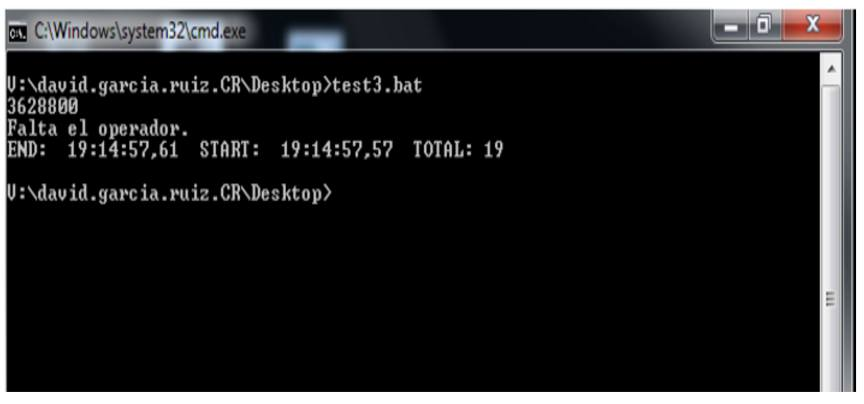
\includegraphics[height=4cm, width=7cm]{factorial_windows7.png}
           \end{tabular}
           & \begin{tabular}{l}
             \parbox{0.5\linewidth}{
	     \begin{itemize}
             \item\textbf{Windows 7}
	     \item\textbf{19 Mil·lisegons}
	     \end{itemize}}
         \end{tabular}  \\
\end{tabular}
}

\frame {
  \frametitle{Comparativa de tiempos/recursos para una aplicación en el mismo PC bajo distintos SO}
  \framesubtitle{Simulació 1 - Factorial}
  \begin{itemize}
  \item\textbf{openSUSE}
	  \begin{itemize}
	  \item{4 Mil·lisegons}
	  \end{itemize}
  \item\textbf{Windows 7}
	  \begin{itemize}
	  \item{19 Mil·lisegons}
	  \end{itemize}
   \end{itemize}
}

\frame {
    \frametitle{Comparativa de rendimiento para una aplicación en el mismo PC bajo distintos SO}
    \framesubtitle{Simulació 2 - Linpack Benchmark}
    \begin{itemize}
    \item {Sistemes operatius:}
	\begin{itemize}
	\item\textbf{openSUSE 13.2 (Harlequin) (64 bits)}
    	\item\textbf{Windows 7 ENTERPRISE (64 bits)}
    	\end{itemize}
    \item {Medició:}
	\begin{itemize}
	\item\textbf{Linpack Benchmark}
    	\end{itemize}
    \item {Processador:}
	\begin{itemize}
	\item\textbf{Intel(R) Core(TM) i5-3470 CPU @ 3.20GHz - 64 bits}
    	\end{itemize}
    \item {Memòria RAM:}
	\begin{itemize}
	\item\textbf{8 GB}
    	\end{itemize}
    \item {Nom de l'equip:}
	\begin{itemize}
	\item\textbf{c6s301pc42}
    	\end{itemize}
    \item {Domini:}
	\begin{itemize}
	\item\textbf{FIBSMB}
    	\end{itemize}
    \end{itemize}
}
\frame {
    \frametitle{Comparativa de rendimiento para una aplicación en el mismo PC bajo distintos SO}
    \framesubtitle{Simulació 2 - Linpack Benchmark}

  \begin{tabular}{cl}  
         \begin{tabular}{c}
           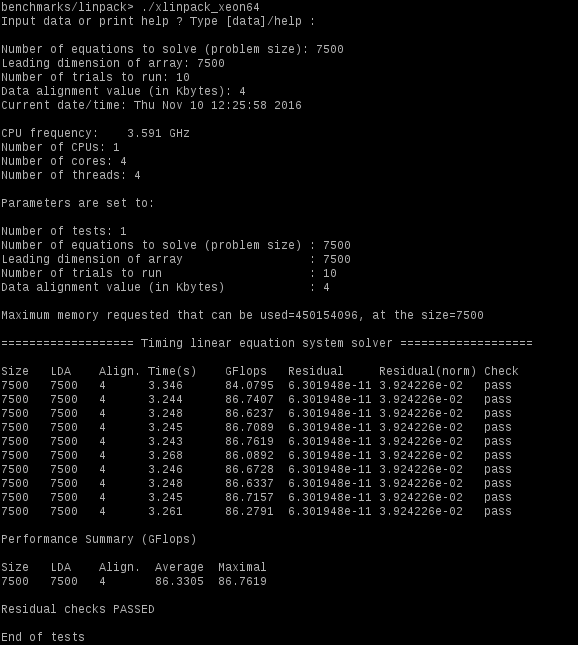
\includegraphics[height=7cm, width=6cm]{linpack_linux.png}
           \end{tabular}
           & \begin{tabular}{l}
             \parbox{0.5\linewidth}{
	     \begin{itemize}
             \item\textbf{openSUSE}
	     \item\textbf{Matrius 7500x7500}
	     \item\textbf{Promig 10 proves}
	     \end{itemize}}
         \end{tabular}  \\
\end{tabular}
}
\frame {
    \frametitle{Comparativa de rendimiento para una aplicación en el mismo PC bajo distintos SO}
    \framesubtitle{Simulació 2 - Linpack Benchmark}

  \begin{tabular}{cl}  
         \begin{tabular}{c}
           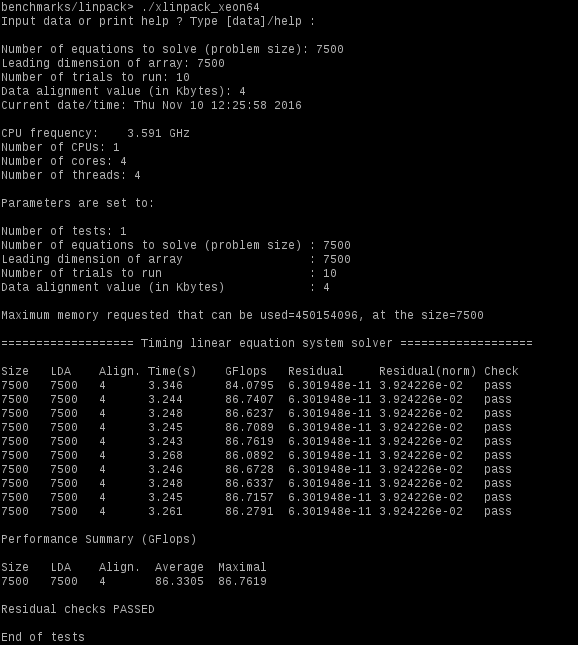
\includegraphics[height=7cm, width=6cm]{linpack_linux.png}
           \end{tabular}
           & \begin{tabular}{l}
             \parbox{0.5\linewidth}{
	     \begin{itemize}
             \item\textbf{openSUSE}
	     \item\textbf{Matrius 7500x7500}
	     \item\textbf{Promig 10 proves}
	     \item\textbf{86.3305 GFLOPS}
	     \end{itemize}}
         \end{tabular}  \\
\end{tabular}
}
\frame {
    \frametitle{Comparativa de rendimiento para una aplicación en el mismo PC bajo distintos SO}
    \framesubtitle{Simulació 2 - Linpack Benchmark}

  \begin{center} 
    \begin{figure}
           \centering
           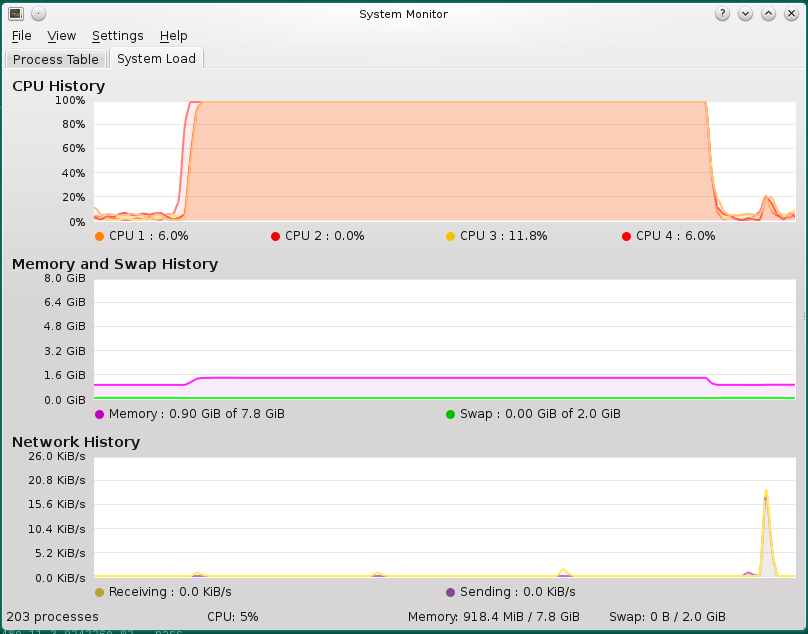
\includegraphics[height=6cm, width=8cm]{linuxmonitor.png}
           \caption{Monitor CPU Linux}
    \end{figure}
  \end{center}
  
}
\frame {
    \frametitle{Comparativa de rendimiento para una aplicación en el mismo PC bajo distintos SO}
    \framesubtitle{Simulació 2 - Linpack Benchmark}

  \begin{tabular}{cl}  
         \begin{tabular}{c}
           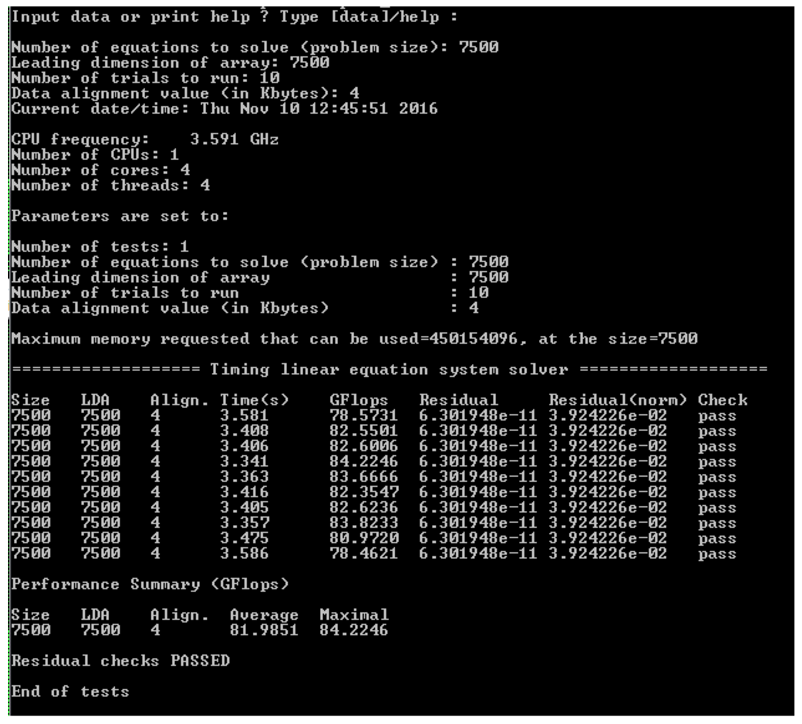
\includegraphics[height=7cm, width=6cm]{linpack_windows.png}
           \end{tabular}
           & \begin{tabular}{l}
             \parbox{0.5\linewidth}{
	     \begin{itemize}
             \item\textbf{Windows 7}
	     \item\textbf{Matrius 7500x7500}
	     \item\textbf{Promig 10 proves}
	     \end{itemize}}
         \end{tabular}  \\
\end{tabular}
}
\frame {
    \frametitle{Comparativa de rendimiento para una aplicación en el mismo PC bajo distintos SO}
    \framesubtitle{Simulació 2 - Linpack Benchmark}

  \begin{tabular}{cl}  
         \begin{tabular}{c}
           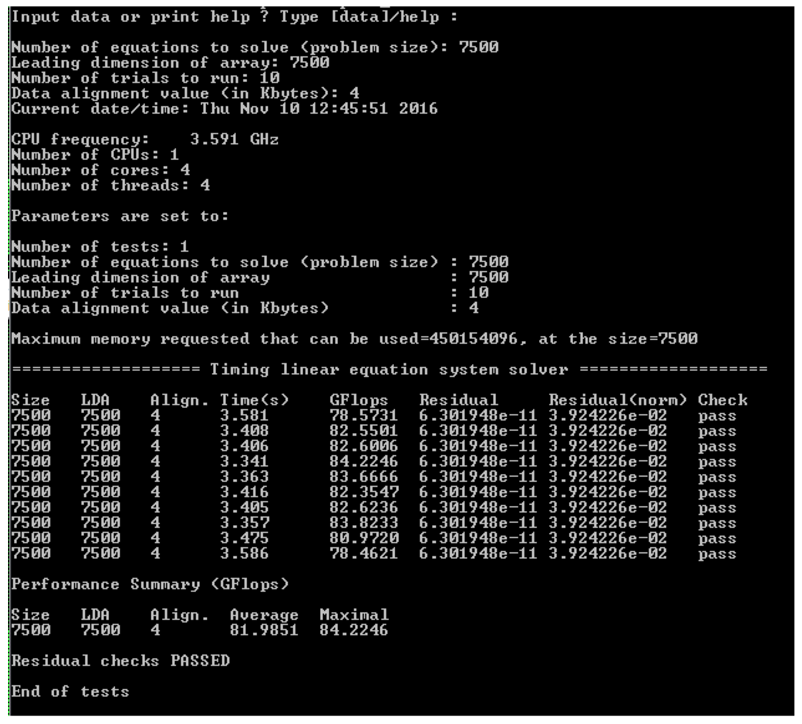
\includegraphics[height=7cm, width=6cm]{linpack_windows.png}
           \end{tabular}
           & \begin{tabular}{l}
             \parbox{0.5\linewidth}{
	     \begin{itemize}
             \item\textbf{openSUSE}
	     \item\textbf{Matrius 7500x7500}
	     \item\textbf{Promig 10 proves}
	     \item\textbf{81.951 GFLOPS}
	     \end{itemize}}
         \end{tabular}  \\
\end{tabular}
}
\frame {
  \frametitle{Comparativa de rendimiento para una aplicación en el mismo PC bajo distintos SO}
  \framesubtitle{Simulació 2 - Linpack Benchmark}
  \begin{itemize}
  \item\textbf{openSUSE}
	  \begin{itemize}
	  \item{86.3305 GFLOPS}
	  \end{itemize}
  \item\textbf{Windows 7}
	  \begin{itemize}
	  \item{81.951 GFLOPS}
	  \end{itemize}
   \end{itemize}
}

\frame {
    \frametitle{Comparativa de tiempos/recursos para una aplicación en el mismo PC bajo distintos SO}
    \framesubtitle{Simulació 3 - Firefox}
    \begin{itemize}
    \item {Sistemes operatius:}
	\begin{itemize}
	\item\textbf{openSUSE 13.2 (Harlequin) (64 bits)}
    	\item\textbf{Windows 7 ENTERPRISE (64 bits)}
    	\end{itemize}
    \item {Medició:}
	\begin{itemize}
	\item\textbf{Firefox}
    	\end{itemize}
    \item {Processador:}
	\begin{itemize}
	\item\textbf{Intel(R) Core(TM) i5-3470 CPU @ 3.20GHz - 64 bits}
    	\end{itemize}
    \item {Memòria RAM:}
	\begin{itemize}
	\item\textbf{8 GB}
    	\end{itemize}
    \item {Nom de l'equip:}
	\begin{itemize}
	\item\textbf{c6s301pc42}
    	\end{itemize}
    \item {Domini:}
	\begin{itemize}
	\item\textbf{FIBSMB}
    	\end{itemize}
    \end{itemize}
}

\begin{frame}[fragile]
\frametitle{Comparativa de tiempos/recursos para una aplicación en el mismo PC bajo distintos SO}
\framesubtitle{Simulació 3 - Firefox}
\textbf{openSUSE}	     
  \begin{lstlisting}
 #!/bin/bash
	START="$(($(date +%s%N)/1000000))"
	firefox "http://www.google.com/" &
	END="$(($(date +%s%N)/1000000))" 
	TOTAL=$(($END-$START))
	echo "END: "$END "START: "$START "TOTAL: "$TOTAL
    \end{lstlisting}
\end{frame}

\frame {
    \frametitle{Comparativa de tiempos/recursos para una aplicación en el mismo PC bajo distintos SO}
    \framesubtitle{Simulació 3 - Firefox}

  \begin{tabular}{cl}  
         \begin{tabular}{c}
           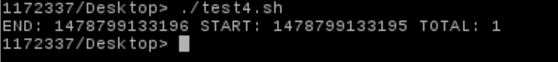
\includegraphics[height=2cm, width=7cm]{firefox_open_suse1.png}
           \end{tabular}
           & \begin{tabular}{l}
             \parbox{0.5\linewidth}{
	     \begin{itemize}
             \item\textbf{openSUSE}
	     \item\textbf{1 Mil·lisegon}
	     \end{itemize}}
         \end{tabular}  \\
\end{tabular}
}

\begin{frame}[fragile]
\frametitle{Comparativa de tiempos/recursos para una aplicación en el mismo PC bajo distintos SO}
\framesubtitle{Simulació 3 - Firefox}
\textbf{Windows 7}	     
  \begin{lstlisting}
 @ECHO OFF
SET START= %time% 
start firefox http://google.com
SET END= %time% 
SET /a TOTAL = %END% - %START%
ECHO END:} %END% START: %START% TOTAL: %TOTAL%
    \end{lstlisting}
\end{frame}

\frame {
    \frametitle{Comparativa de tiempos/recursos para una aplicación en el mismo PC bajo distintos SO}
    \framesubtitle{Simulació 3 - Firefox}

  \begin{tabular}{cl}  
         \begin{tabular}{c}
           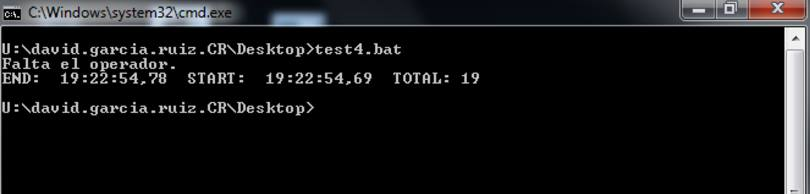
\includegraphics[height=2.5cm, width=7cm]{firefox-windows.png}
           \end{tabular}
           & \begin{tabular}{l}
             \parbox{0.5\linewidth}{
	     \begin{itemize}
             \item\textbf{Windows 7}
	     \item\textbf{19 Mil·lisegons}
	     \end{itemize}}
         \end{tabular}  \\
\end{tabular}
}
\frame {
  \frametitle{Comparativa de tiempos/recursos para una aplicación en el mismo PC bajo distintos SO}
  \framesubtitle{Simulació 3 - Firefox}
  \begin{itemize}
  \item\textbf{openSUSE}
	  \begin{itemize}
	  \item{1 Mil·lisegon}
	  \end{itemize}
  \item\textbf{Windows 7}
	  \begin{itemize}
	  \item{19 Mil·lisegons}
	  \end{itemize}
   \end{itemize}
}
\frame {
  \frametitle{Comparativa de tiempos/recursos para una aplicación en el mismo PC bajo distintos SO}
  \framesubtitle{Conclusions Simulacions}
  \begin{itemize}
  	\item\ No únicament el SO afecta en els temps/recursos
  	\item\ Hi ha \textbf{"Soroll"} que afecta
  	\item\ Identificar que ocasiona "Soroll"
   \end{itemize}
}
\frame {
  \frametitle{Comparativa de tiempos/recursos para una aplicación en el mismo PC bajo distintos SO}
  \framesubtitle{Alternatives millora rendiment SO}
  \begin{itemize}
  	\item\textbf{Windows} 
  	\item\ Pot funcionar més lent del que s'espera
  	\item\ Disc dur més ple del que es recomana
   \end{itemize}
}
\frame {
  \frametitle{Comparativa de tiempos/recursos para una aplicación en el mismo PC bajo distintos SO}
  \framesubtitle{Alternatives millora rendiment SO}
  \begin{itemize}
  	\item\textbf{Windows} 
  	\item\ Tenir més Memòria RAM amb eines com \textbf{ReadyBoost}
  	\item\ Desactivar serveis:
  	\begin{itemize}
            \item Application experience
            \item Computer browser
            \item Security server
  	\end{itemize}
   \end{itemize}
}

\frame {
    \frametitle{Comparativa de tiempos/recursos para una aplicación en el mismo PC bajo distintos SO}
    \framesubtitle{Alternatives millora rendiment SO}

  \begin{tabular}{cl}  
         \begin{tabular}{c}
       %  \begin{figure}
           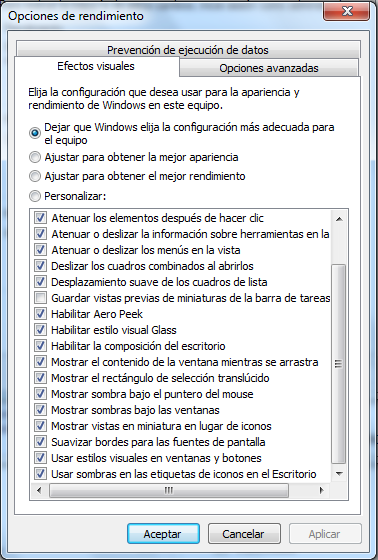
\includegraphics[height=6cm, width=5cm]{efectos_visuales.png}
         %  \caption{Efectos Visuales Windows 7}
        % \end{figure}
           \end{tabular}
           & \begin{tabular}{l}
             \parbox{0.5\linewidth}{
	     \begin{itemize}
             \item{Desactivar efectes visuals}
	     \end{itemize}}
         \end{tabular}  \\
\end{tabular}
}
\frame {
    \frametitle{Comparativa de tiempos/recursos para una aplicación en el mismo PC bajo distintos SO}
    \framesubtitle{Alternatives millora rendiment SO}

  \begin{tabular}{cl}  
         \begin{tabular}{c}
           \includegraphics[height=3cm, width=2.5cm]{desactivar-uac.png}
         %  \caption{Control de cuentas de usuarios de Windows 7}
           \end{tabular}
           & \begin{tabular}{l}
             \parbox{0.5\linewidth}{
	     \begin{itemize}
             \item{Desactivar UAC \\(Control Cuentas Usuario)}
	     \end{itemize}}
         \end{tabular}  \\
\end{tabular}
}

\frame {
    \frametitle{Comparativa de tiempos/recursos para una aplicación en el mismo PC bajo distintos SO}
    \framesubtitle{Alternatives millora rendiment SO}

  \begin{center} 
    \begin{figure}
           \centering
           \includegraphics[height=5cm, width=7cm]{liberador-espacio-windows.png}
           \caption{Alliberador d'espai en disc Windows 7}
    \end{figure}
  \end{center}
}
\frame {
    \frametitle{Comparativa de tiempos/recursos para una aplicación en el mismo PC bajo distintos SO}
    \framesubtitle{Alternatives millora rendiment SO}

  \begin{center} 
    \begin{figure}
           \centering
           \includegraphics[height=5cm, width=7cm]{duplicate.png}
           \caption{Duplicate File Finder}
    \end{figure}
  \end{center}
}
\frame {
    \frametitle{Comparativa de tiempos/recursos para una aplicación en el mismo PC bajo distintos SO}
    \framesubtitle{Alternatives millora rendiment SO}

  \begin{center} 
    \begin{figure}
           \centering
           \includegraphics[height=5cm, width=7cm]{ccleaner.png}
           \caption{CCleaner}
    \end{figure}
  \end{center}
}
\frame {
  \frametitle{Comparativa de tiempos/recursos para una aplicación en el mismo PC bajo distintos SO}
  \framesubtitle{Alternatives millora rendiment SO}
  \begin{itemize}
  	\item\textbf{openSUSE} 
  	\item\ Actualitzar el Kernel
  	\item\ Desactivar efectes especials
        \item\ Desinstalar aplicacions no utilitzades 
   \end{itemize}
}
\frame {
    \frametitle{Comparativa de tiempos/recursos para una aplicación en el mismo PC bajo distintos SO}
    \framesubtitle{Alternatives millora rendiment SO}

  \begin{center} 
    \begin{figure}
           \centering
           \includegraphics[height=5cm, width=7cm]{desactivar-aplicaciones-linux.png}
           \caption{Preferencias aplicaciones instaladas en Linux}
    \end{figure}
  \end{center}
}
\frame {
    \frametitle{Comparativa de tiempos/recursos para una aplicación en el mismo PC bajo distintos SO}
    \framesubtitle{Alternatives millora rendiment SO}

  \begin{center} 
    \begin{figure}
           \centering
           \includegraphics[height=5cm, width=7cm]{limpieza-linux-synaptic.png}
           \caption{Synaptic Package Manager}
    \end{figure}
  \end{center}
}
\frame {
    \frametitle{Comparativa de tiempos/recursos para una aplicación en el mismo PC bajo distintos SO}
    \framesubtitle{Alternatives millora rendiment SO}

  \begin{center} 
    \begin{figure}
           \centering
           \includegraphics[height=5cm, width=7cm]{limpieza-linux-beatbit.png}
           \caption{BleachBit}
    \end{figure}
  \end{center}
}



% End Arnau Garcia
% Begin Guillem Gordillo

\frame {
    \frametitle{Posibilidades de simulación / virtualización en unos y otros. Interoperabilidad}
    \textbf{Guillem Gordillo}
}

% End Guillem Gordillo
\small
\frame {
    \frametitle{Bibliografia}
    \begin{itemize}
        \item {http://informatica.blogs.uoc.edu/2016/03/08/guia-para-elegir-el-sistema-operativo-de-tu-ordenador-windows-os-x-o-linux/}
        \item {http://www.howtogeek.com/197559/how-to-install-windows-10-on-your-pc/}
        \item {https://help.ubuntu.com/community/Installation}
        \item {https://support.apple.com/en-us/HT204904}
        \item {http://venturebeat.com/2016/03/30/hey-microsoft-how-many-apps-are-in-the-windows-store/}
        \item {https://wiki.ubuntu.com/SoftwareCenter}
    \end{itemize}
}

\frame {
    \frametitle{Bibliografia}
    \begin{itemize}
        \item {https://www.rootusers.com/windows-nfs-vs-linux-nfs-performance-comparison/}
        \item {http://rootear.com/windows/alternativa-admin-windows}
        \item {http://es.ccm.net/faq/3435-linux-comandos-para-monitorear-el-sistema}
        \item {http://www.genbeta.com/linux/como-monitorizar-constantemente-el-rendimiento-de-tu-distro-gnu-linux}
        \item {https://www.atareao.es/ubuntu/ahorra-recursos-y-bateria-en-chrome-con-the-great-suspender-en-ubuntu/}
        \item {http://elblogdeliher.com/como-instalar-y-configurar-conky-en-ubuntu/}        
    \end{itemize}
}

\frame {
    \frametitle{Bibliografia}
    \begin{itemize}
        \item {http://www.applesfera.com/aplicaciones-os-x-1/monitor-de-actividad-y-otras-aplicaciones-para-monitorizar-nuestro-mac}
        \item {https://support.apple.com/es-es/HT201538}
        \item {https://bjango.com/mac/istatmenus/}
        \item {https://itunes.apple.com/us/app/statsbar-system-monitor/}
        \item {https://support.apple.com/en-us/HT201475}
        \item {http://www.macworld.co.uk/how-to/mac-software/how-run-os-x-on-pc-3632329/}
        \item {https://www.rootusers.com/windows-nfs-vs-linux-nfs-performance-comparison/}
        \item {http://www.tuxradar.com/content/benchmarked-ubuntu-vs-vista-vs-windows-7}
    \end{itemize}
}


\end{document}
